\documentclass{article}
\usepackage[margin=1in]{geometry}
\usepackage{siunitx}
\usepackage{array}
\usepackage{booktabs}
\usepackage{hyperref}
\usepackage{graphicx}
\usepackage{amsmath}

\begin{document}
\author{Sachith Dunatunga}
\title{16.930 PS4}
\maketitle

\section{Q1}
Surprisingly, the answer is provided in the reference material\cite{nguyen}.
The choice of $\tau$ which reduces to the regular DG method is given by
\begin{align}
\tau = \frac{1}{2} \left( | \mathbf{c} \cdot \mathbf{n} | + \mathbf{c} \cdot \mathbf{n} \right)
\end{align}

\section{Convergence plots for Structured Case}
I am sorry about this, but I realized too late that I followed the notes a bit too closely and subsequently $\mathbf{q}$ approximates $\kappa \nabla u$ instead of $\nabla u$.
Happily, this does not affect this test in particular (since $\kappa = 1$).
The postprocessing also assumes $\kappa = 1$, since I did not want to modify the function signature, so it truly is applied on the gradient of $u$.

In figure \ref{fig:cs} we see the expected convergence behavior (p+1) for u when selecting $\tau = 1$ or $1/h$.
However, the rate drops to order p for $\tau = h$.

Interestingly, we see the expected convergence behaviors for $q_x$ and $q_y$ when selecting $\tau = 1$ or $\tau = h$, but the rate drops to order p for $\tau = 1/h$.

Since the postprocessing step relies on the order of $\mathbf{q}$ and $u$, it then makes sense that $\tau = 1$ results in a p+2 convergence rate for $u^*$. I was surprised that $\tau = h$ also had this p+2 rate (since u was order p), but I was not surprised that $\tau = 1/h$ would result in staying at order p+1 for $u^*$.

\begin{figure}
\begin{tabular}{c c c}
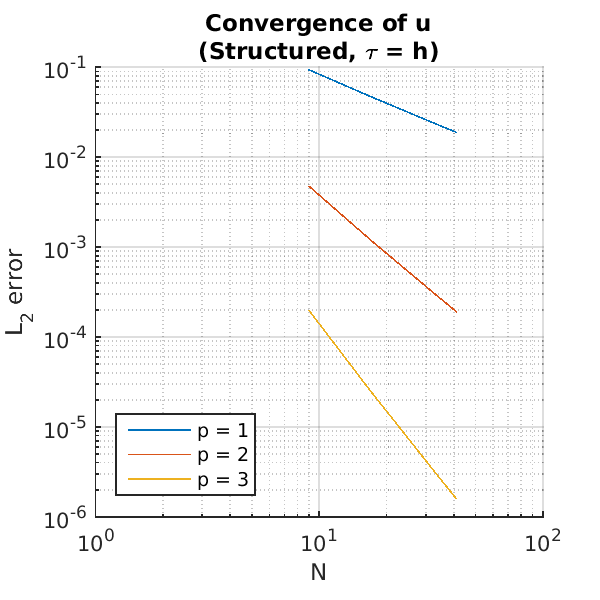
\includegraphics[scale=0.5]{cs_1.png} & 
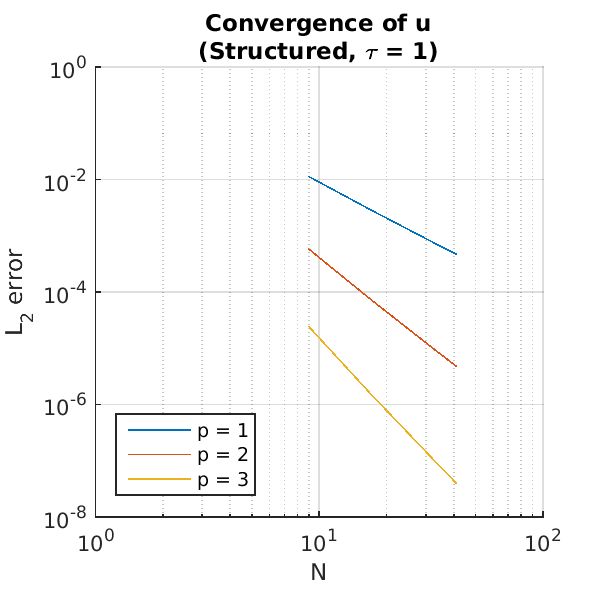
\includegraphics[scale=0.5]{cs_2.png} & 
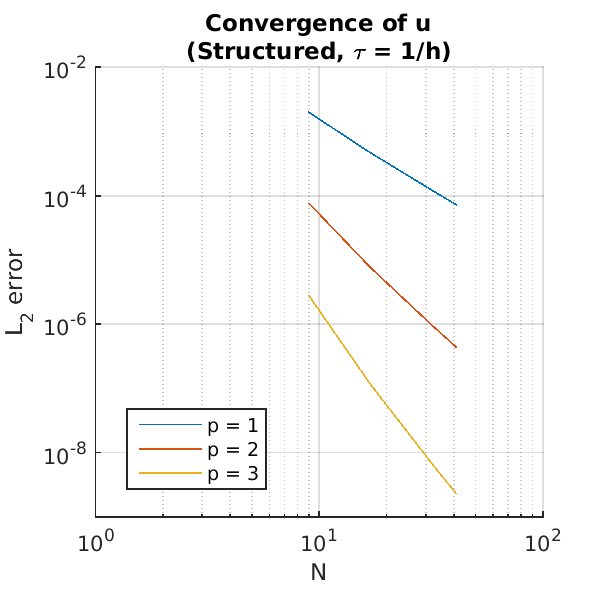
\includegraphics[scale=0.5]{cs_3.png} \\
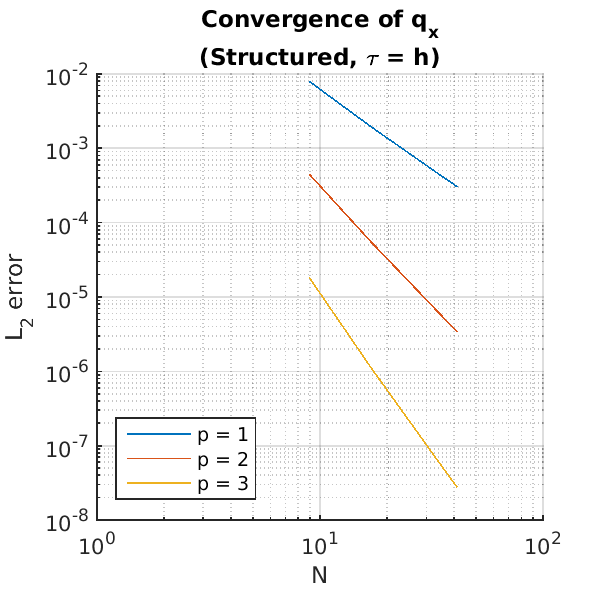
\includegraphics[scale=0.5]{csqx_1.png} & 
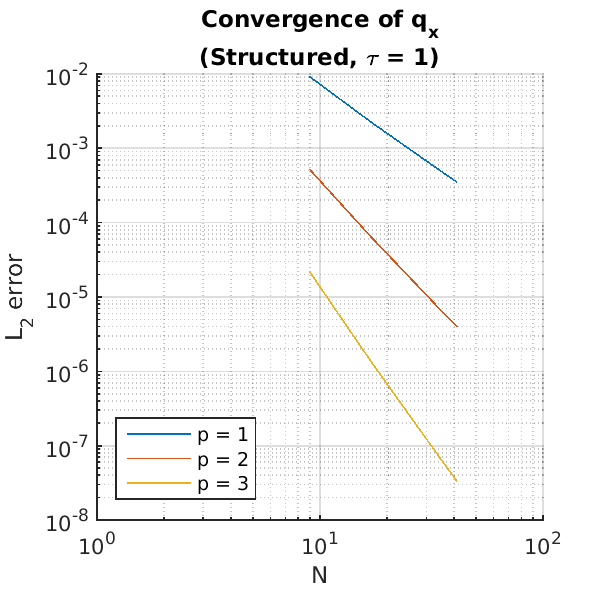
\includegraphics[scale=0.5]{csqx_2.png} & 
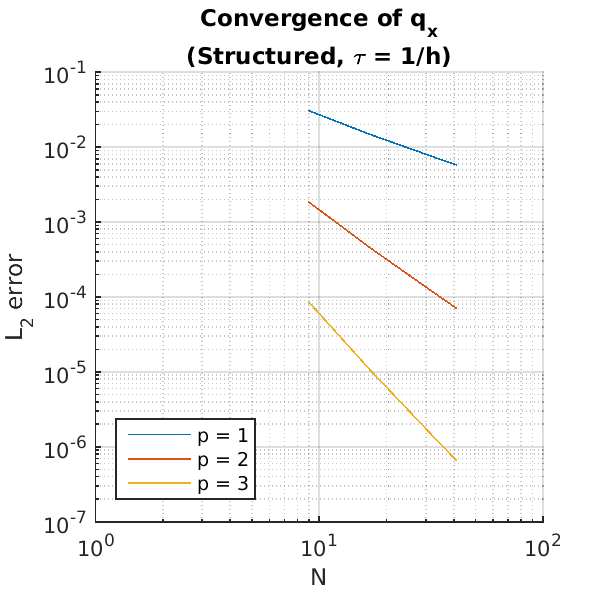
\includegraphics[scale=0.5]{csqx_3.png} \\
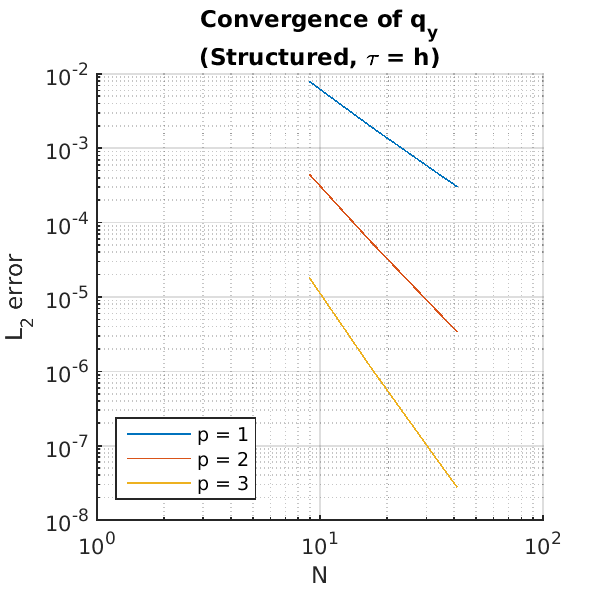
\includegraphics[scale=0.5]{csqy_1.png} & 
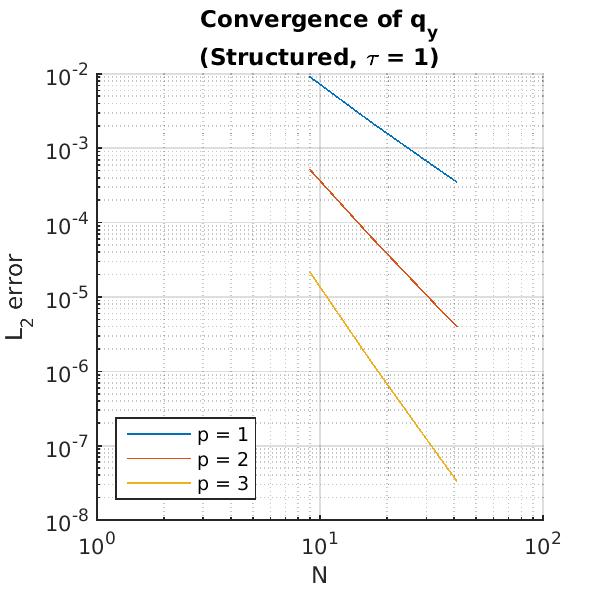
\includegraphics[scale=0.5]{csqy_2.png} & 
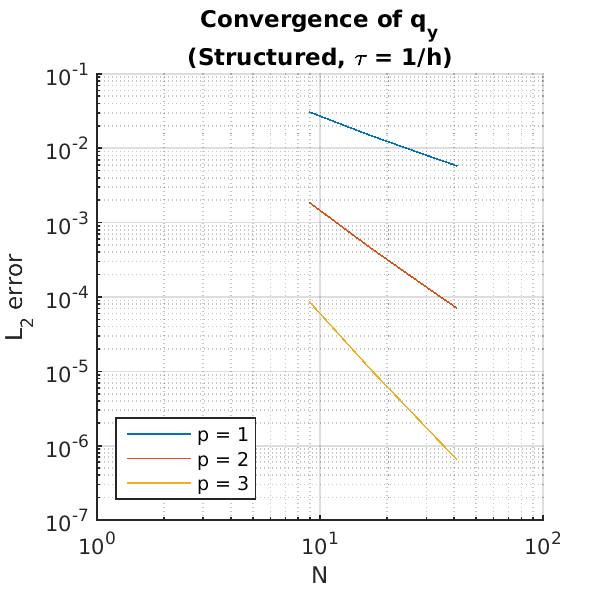
\includegraphics[scale=0.5]{csqy_3.png} \\
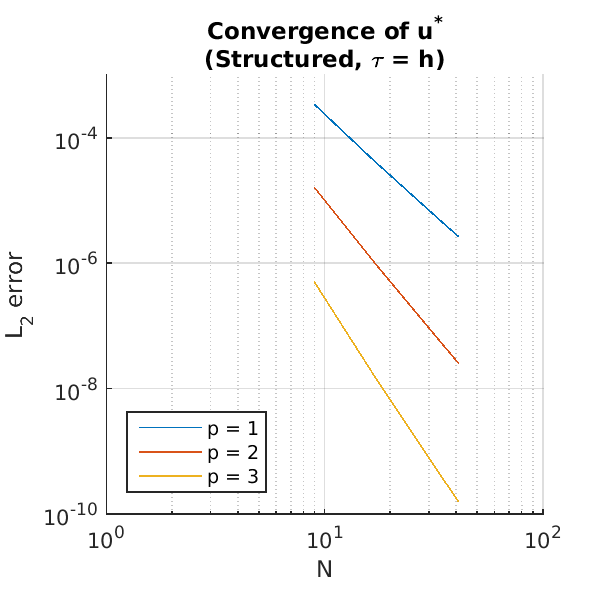
\includegraphics[scale=0.5]{cspp_1.png} & 
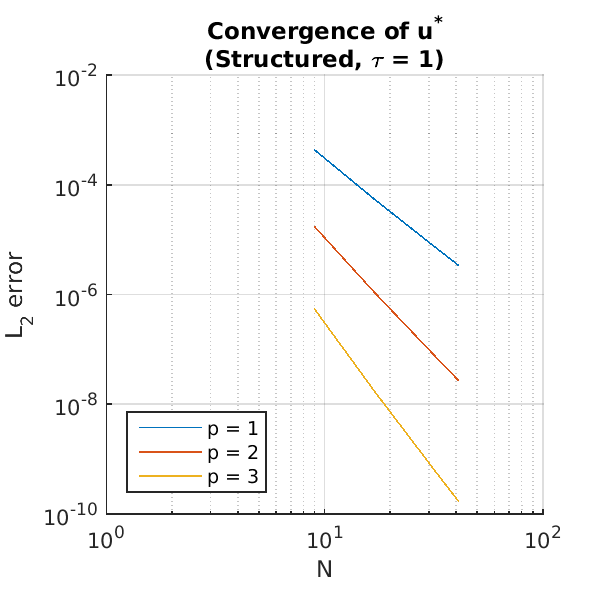
\includegraphics[scale=0.5]{cspp_2.png} & 
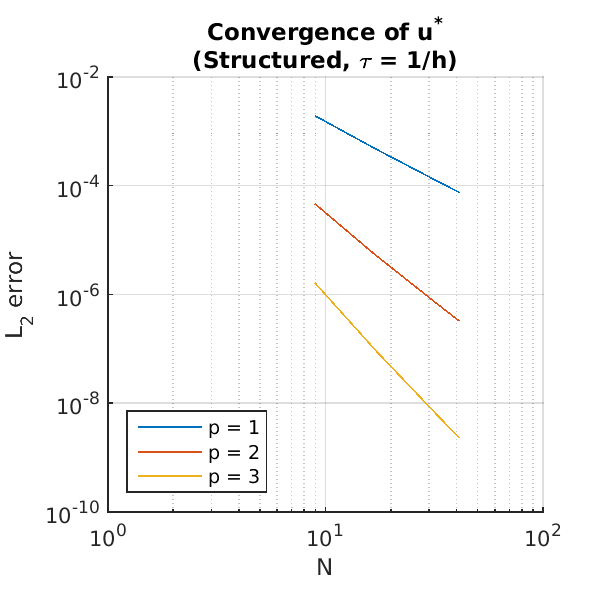
\includegraphics[scale=0.5]{cspp_3.png}
\end{tabular}
\label{fig:cs}
\caption{Convergence plots on the structured mesh. We have the stabilizations $\tau = h, 1, 1/h$ from left to right. The variables we compare are $u, q_x, q_y, u^*$ from top to bottom. We only get good convergence for everything when $\tau = 1$.}
\end{figure}

I did not have time to convert this to a proper table, but doing a linear fit of the last couple points confirms our code is working for the diffusion case.
I went out to 40 elements in addition to the specified 8, 16, and 32 sizes (convergence was higher than I expected with just the 3 meshes, but it appears to have been a transient effect, since the rate went back down by adding the even finer mesh).
The series below includes this mesh with n=40.
\begin{verbatim}
u
h - Order 1 has rate -1.02711.
h - Order 2 has rate -2.0551.
h - Order 3 has rate -3.08317.
1 - Order 1 has rate -2.04695.
1 - Order 2 has rate -3.07596.
1 - Order 3 has rate -4.10484.
1/h - Order 1 has rate -2.06656.
1/h - Order 2 has rate -3.13457.
1/h - Order 3 has rate -4.25809.
qx
h - Order 1 has rate -2.05846.
h - Order 2 has rate -3.08746.
h - Order 3 has rate -4.11365.
1 - Order 1 has rate -2.06695.
1 - Order 2 has rate -3.09276.
1 - Order 3 has rate -4.12155.
1/h - Order 1 has rate -1.03401.
1/h - Order 2 has rate -2.05983.
1/h - Order 3 has rate -3.08649.
qy
h - Order 1 has rate -2.05846.
h - Order 2 has rate -3.08746.
h - Order 3 has rate -4.11365.
1 - Order 1 has rate -2.06695.
1 - Order 2 has rate -3.09276.
1 - Order 3 has rate -4.12156.
1/h - Order 1 has rate -1.03401.
1/h - Order 2 has rate -2.05983.
1/h - Order 3 has rate -3.08649.
u*
h - Order 1 has rate -3.08705.
h - Order 2 has rate -4.11205.
h - Order 3 has rate -5.14057.
1 - Order 1 has rate -3.08851.
1 - Order 2 has rate -4.11603.
1 - Order 3 has rate -5.1444.
1/h - Order 1 has rate -2.05619.
1/h - Order 2 has rate -3.09672.
1/h - Order 3 has rate -4.12233.
\end{verbatim}

\begin{thebibliography}{9}
\bibitem{nguyen}
N.C. Nguyen, J. Peraire, B. Cockburn
\textit{An implicit high-order hybridizable discontinuous Galerkin method for linear convection-diffusion equations}
Journal of Computational Physics, 228 (2009) 3232-3254
\end{thebibliography}

\end{document}
